\documentclass[conference]{IEEEtran}
\IEEEoverridecommandlockouts
% The preceding line is only needed to identify funding in the first footnote. If that is unneeded, please comment it out.
\usepackage{cite}
\usepackage{amsmath,amssymb,amsfonts}
\usepackage{algorithmic}
\usepackage{graphicx}
\usepackage{textcomp}
\usepackage{xcolor}
\usepackage{float}

\def\BibTeX{{\rm B\kern-.05em{\sc i\kern-.025em b}\kern-.08em
    T\kern-.1667em\lower.7ex\hbox{E}\kern-.125emX}}
\begin{document}

\title{Detection of heart anomalies by use of adaptive LMS filters in ECG signals*\\
{\footnotesize \textsuperscript{*}Note: Sub-titles are not captured in Xplore and
should not be used}
}

\author{\IEEEauthorblockN{1\textsuperscript{st} Tom\'as Agust\'in Gonz\'alez Orlando}
\IEEEauthorblockA{\textit{Procesamiento Adaptativo de Se\~nales} \\
\textit{Instituto Tecnológico de Buenos Aires}\\
Buenos Aires, Argentina\\
togonzalez@itba.edu.ar}
\and
\IEEEauthorblockN{2\textsuperscript{nd} Ariel Santiago Nowik}
\IEEEauthorblockA{\textit{Procesamiento Adaptativo de Se\~nales} \\
\textit{Instituto Tecnológico de Buenos Aires}\\
Buenos Aires, Argentina\\
anowik@itba.edu.ar}
}

\maketitle

\begin{abstract}
An implementation of a heart anomaly detector for non-paced rhythms using different adaptive filter structures is proposed.\par
The detection algorithm uses an Adaptive Recursive Filter (ARF), for which the impulse input is previously determined via a peak localization and time shift estimation algorithm. \par
The detection of each anomaly by itself is product of the direct observation of the magnitude of the ARF output.
The design and testing of the detector was based on the MIT-BIH Arrhythmia Database with almost none false-negative and few false-positive results.
\end{abstract}

\begin{IEEEkeywords}
ECG analysis, heart anomaly detection, Adaptive Filtering, LMS filters
\end{IEEEkeywords}


\section{Introduction}


\subsection{Electrocardiogram signals}

An Electrocardiogram (ECG) signal is a non invasive recording (electrodes are placed on the patient's skin) of the electrical activity of a heart. There are several places where the signals may be recorded, and usually as many as ten electrodes are used to perform an ECG, where the polarization and repolarization of the heart muscles are recorded. \par
An ECG portrays an incredibly large amount of information from the patient, such as the rate and rhythm of heartbeats, the size and position of the heart chambers, the presence of any damage to the heart's muscle cells or conduction system, the effects of heart drugs, and the function of implanted pacemakers.\par
These polarization cycles form the main three components of a heart signal, which are listed as follows:
\begin{itemize}
\item \underline{P-wave} : Depolarization of the atria. This component is frequently the one with the lowest amplitude.
\item \underline{QRS complex}: Depolarization of the ventricles. In the QRS complex a peak of high frequency and the highest amplitude is detected. 
\item \underline{T-wave}: Repolarization of the ventricles.
\end{itemize} 

\begin{figure}[H]
\centerline{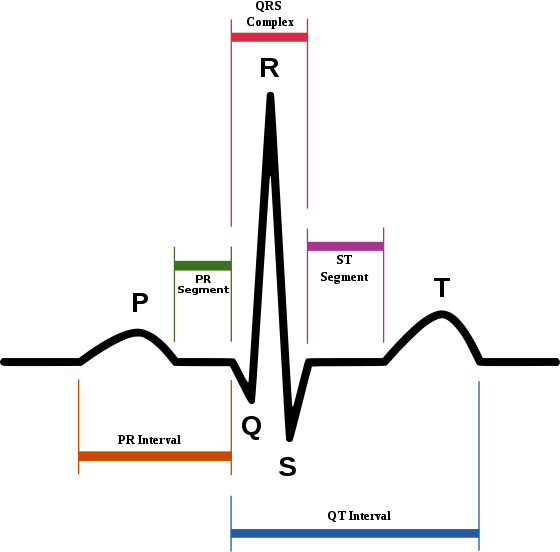
\includegraphics[scale=0.3]{SinusRhythmLabels}}
\caption{Main components of an ECG signal}
\label{fig}
\end{figure}

These components were enumerated in their usual order of appearance. However, some patients with heart abnormalities exhibit a P-wave that superposes over the QRS complex, so the techniques developed below should take into account this factor when analysing the ECG signal even with no previous knowledge of the abnormality. Adaptive filters have been proven efficient in such cases. \par

\subsection{Adaptive Recursive Filters}

An Adaptive Recursive Filter (ARF) is an adaptive filter whose coefficients change so that when it is adapted, its impulse response converges to a single pseudo-period of an ideally periodic signal. The ARF is therefore applied to signals that are known to have periodic behaviour with considerably small changr
s through time in both its pseudo-periods and its fundamental period.\par
The signal in question may be then considered to be stationary between time intervals of a given length.\par
A diagram of the ARF, taken from \cite{b1} is shown below:

\begin{figure}[H]
\centerline{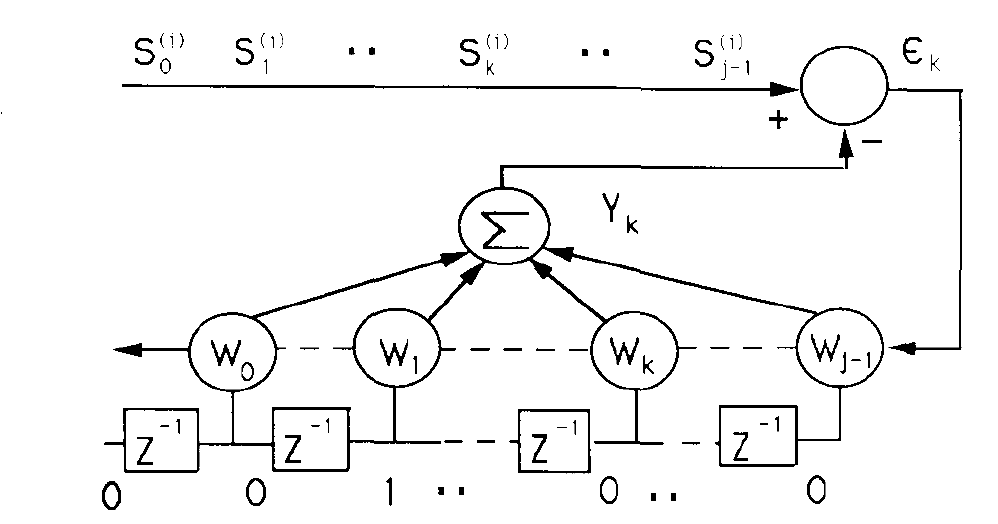
\includegraphics[scale=0.7]{ARF_diagram.png}}
\caption{Basic diagram of an ARF}
\label{fig}
\end{figure}

The ARF has two input signals: \par
The original (ECG) signal and a signal which contains only impulses in the beginning of each pseudo period of the original signal. Via this method, the coefficients of the filter will be updated one by one in each iteration, so that if $w_k$ is the k-th coefficient of the filter, $w_k$ will be updated in one iteration of the algorithm and then  $w_{k+1}$ will be updated in the next iteration. This is because in each iteration, the filter will compare its impulse response at a single time (hence, at a single coefficient) with the input signal at that specific time, and the error derived from that comparison will be fed to the adaptive filter so as to minimize its cost function.

\section{LMS prediction}

The first approach taken was the implementation of an adaptive predictor based on the following diagram:

\begin{figure}[H]
\centerline{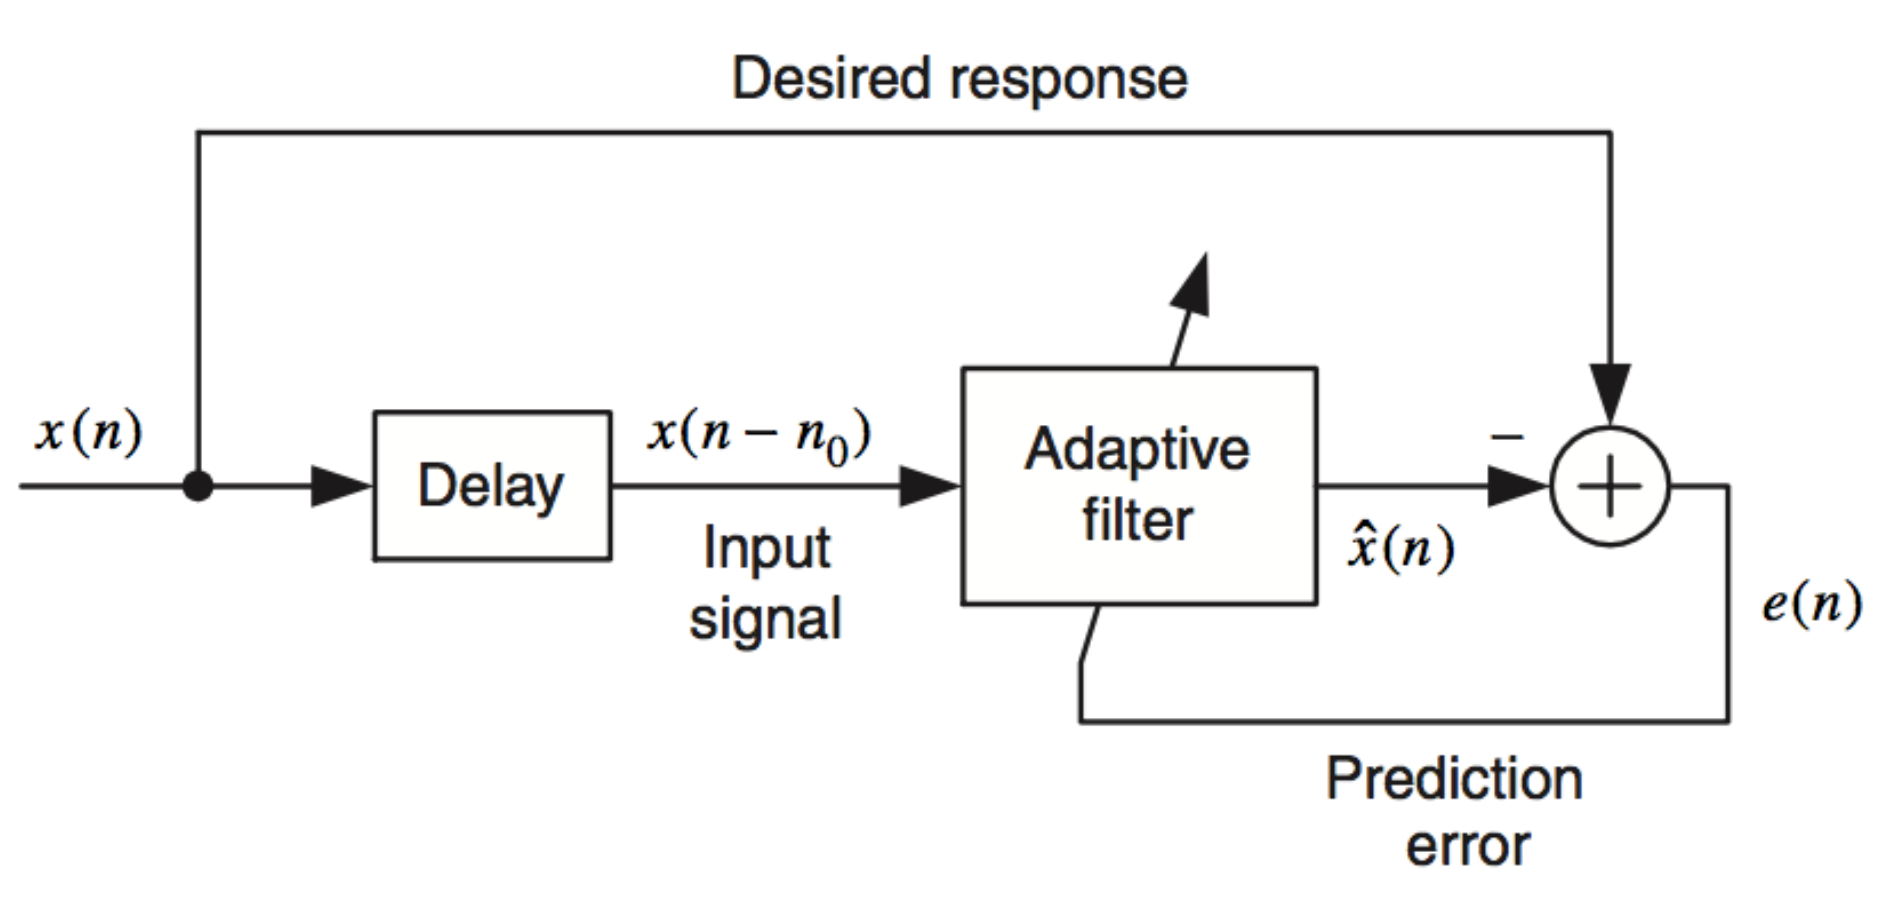
\includegraphics[scale=0.4]{prediction.png}}
\caption{Adaptive predictor diagram}
\label{fig}
\end{figure}

The implementation achieved its desired purpose of predicting the signal, as shown in the following figure:

\begin{figure}[H]
\centerline{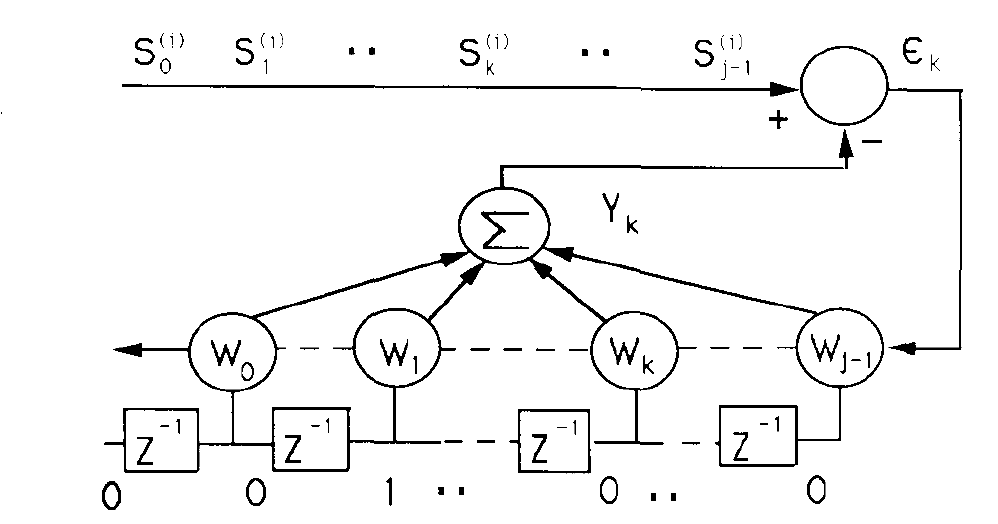
\includegraphics[scale=0.7]{ARF_diagram.png}}
\caption{Signal 202 of the MIT-BIH Arrhythmia Database, minute , and the predictor's response.}
\label{fig}
\end{figure}

The magnitude of the error signal was afterwards processed in order to get its peaks, which where considered anomalies when its amplitude exceeded a designated value. This method of anomaly detection did not manage to achieve acceptable results as the predictor error tends to raise when the ECG signal has high frequency changes, and so the the peaks of the QRS complex were also taken as anomalies. \par
Although this problem disqualified the method, if the QRS complex is detected via a previous analysis of the signal, discarding the false positives that appear with its peaks may be a path to be followed in future investigations.\par

\section{Detection}

The detection of each anomaly consists of applying the detection algorithm to the entire ECG signal or a portion of it. The steps of this algorithm are in line with the arrythmia detection method stated by \cite{b1}:

\begin{enumerate}
\item Find the peaks of each QRS complex.
\item Generate an impulse signal in which each impulse coincides with the beggining of the QRS complex.  
\item Feed the ARF with both the new impulse signal and the ECG. 
\item Get the error signal of the ARF after processing the inputs.
\item Identify the peaks of the absolute error signal and select those points in which these peaks may signify an anomaly.
\end{enumerate}

Choosing to generate an impulse at the start of the QRS complex and not at the start of the P-wave is the solution for the possibility of an abnormality in the P-wave that may provoke it to overlap with other components of the signal. The ARF will make its impulse response copy by default the QRS complex and the T-wave, and in such case that no overlapping ocurrs, the P-wave will also be shown in the impulse response of the filter.

\subsection{Detection of the QRS complex}

The localization of the QRS complex is based on the detection of high amplitude peaks. This may be done by assuming signal stationarity for some interval of time. Fifteen pseudo-periods of the signal has been proven an effective amount of time. The period has been estimated with the a priori knowledge of an ECG: The period of a heart signal is of approximately 1 beat per second. Taking this into account and the fact that the sample rate of the MIT-BIH Database is 360 Hz, a number of 350 samples was the estimated length of a heart beat. \par
After defining the stationary interval, the signal is then converted to its energy signal by simply squaring each value. Converting the signal to its energy signal for peak detection has two advantages:

\begin{enumerate}
\item All values of the energy signal will be non negative.
\item Greater values will be weigthed as more important and significative than smaller values as pondered by the square function.
\end{enumerate}

A peak will be detected each time a sample of the energy signal has a value that is at least 0.55 times the maximum value of the interval.

\subsection{Generation of the impulse signal}

As each peak of the QRS complex corresponds to the R component of the signal, a time shift should be applied so that the generated impulse signal will have its impulse assigned to the beginning of the QRS complex. This time shift should also be estimated in a proportion of the estimated pseudo-period time, although this estimation may also be updated every time a new peak is detected.

\subsection{Design and implementation of the ARF}

The ARF was implemented using the same LMS filter used in the adaptive predictor filter. No variants of the LMS algorithm were used, as its accuracy was more than acceptable. The convergence step $\mu$ of the LMS algorithm was chosen prioritizing the convergence velocity of the algorithm so that the filter could be used in almost real time like applications. With this objective in mind, $\mu$ was firstly given an initial value that made the algorithm unstable and then was decremented until the filter converged for all ECG signals in the database. \par
The ARF filter was fed with the generated impulse signal and the original ECG signal. Although the output signal was available, it was only required to verify that the impulse response of the filter was indeed adapting to the original signal (In the particular case of the ARF, this step is equivalent to coefficient tracking). This was done both graphically and by observation of the error signal and the quadratic error of the filter.\par

\subsection{Baseline Wander and noise handling}

Due to muscle movements and the noise frequencies of the electric line, the signals baseline was variable along time. This caused problems when determining peaks and when analysing the error signal of the ARF, which resulted in the appearance of several false positives, as the impulse signal input of the ARF was corrupted and so the filter could not adapt its coefficients correctly. \par
Numerous methods for reducing the baseline wander were tried, such as:
\begin{itemize}
\item Interference elimination of the line frequency using the common mode between the two available ECG signals as a reference and the analysed signal as input.
\item Non adaptive notch and bandpass filters between 0.7 Hz and 125Hz as stated in \cite{b2}
\item Lineal detrending of the signal.
\end{itemize}

In the end, the use a high-pass filter was the method that proved more successful to remove the baseline wander. 

\section{Criteria for recognizing heart anomalies}
Until now we have developed a system with several stages, first a filter to remove low frequencies trends, then a peak detector. The ARF used peak detector output and signal to build an error signal that would contain information easy to extract to detect anomalies.
So now we will need to make an algorithm that with that signal detect electrocardiogram problems.
\begin{figure}[H]
\centerline{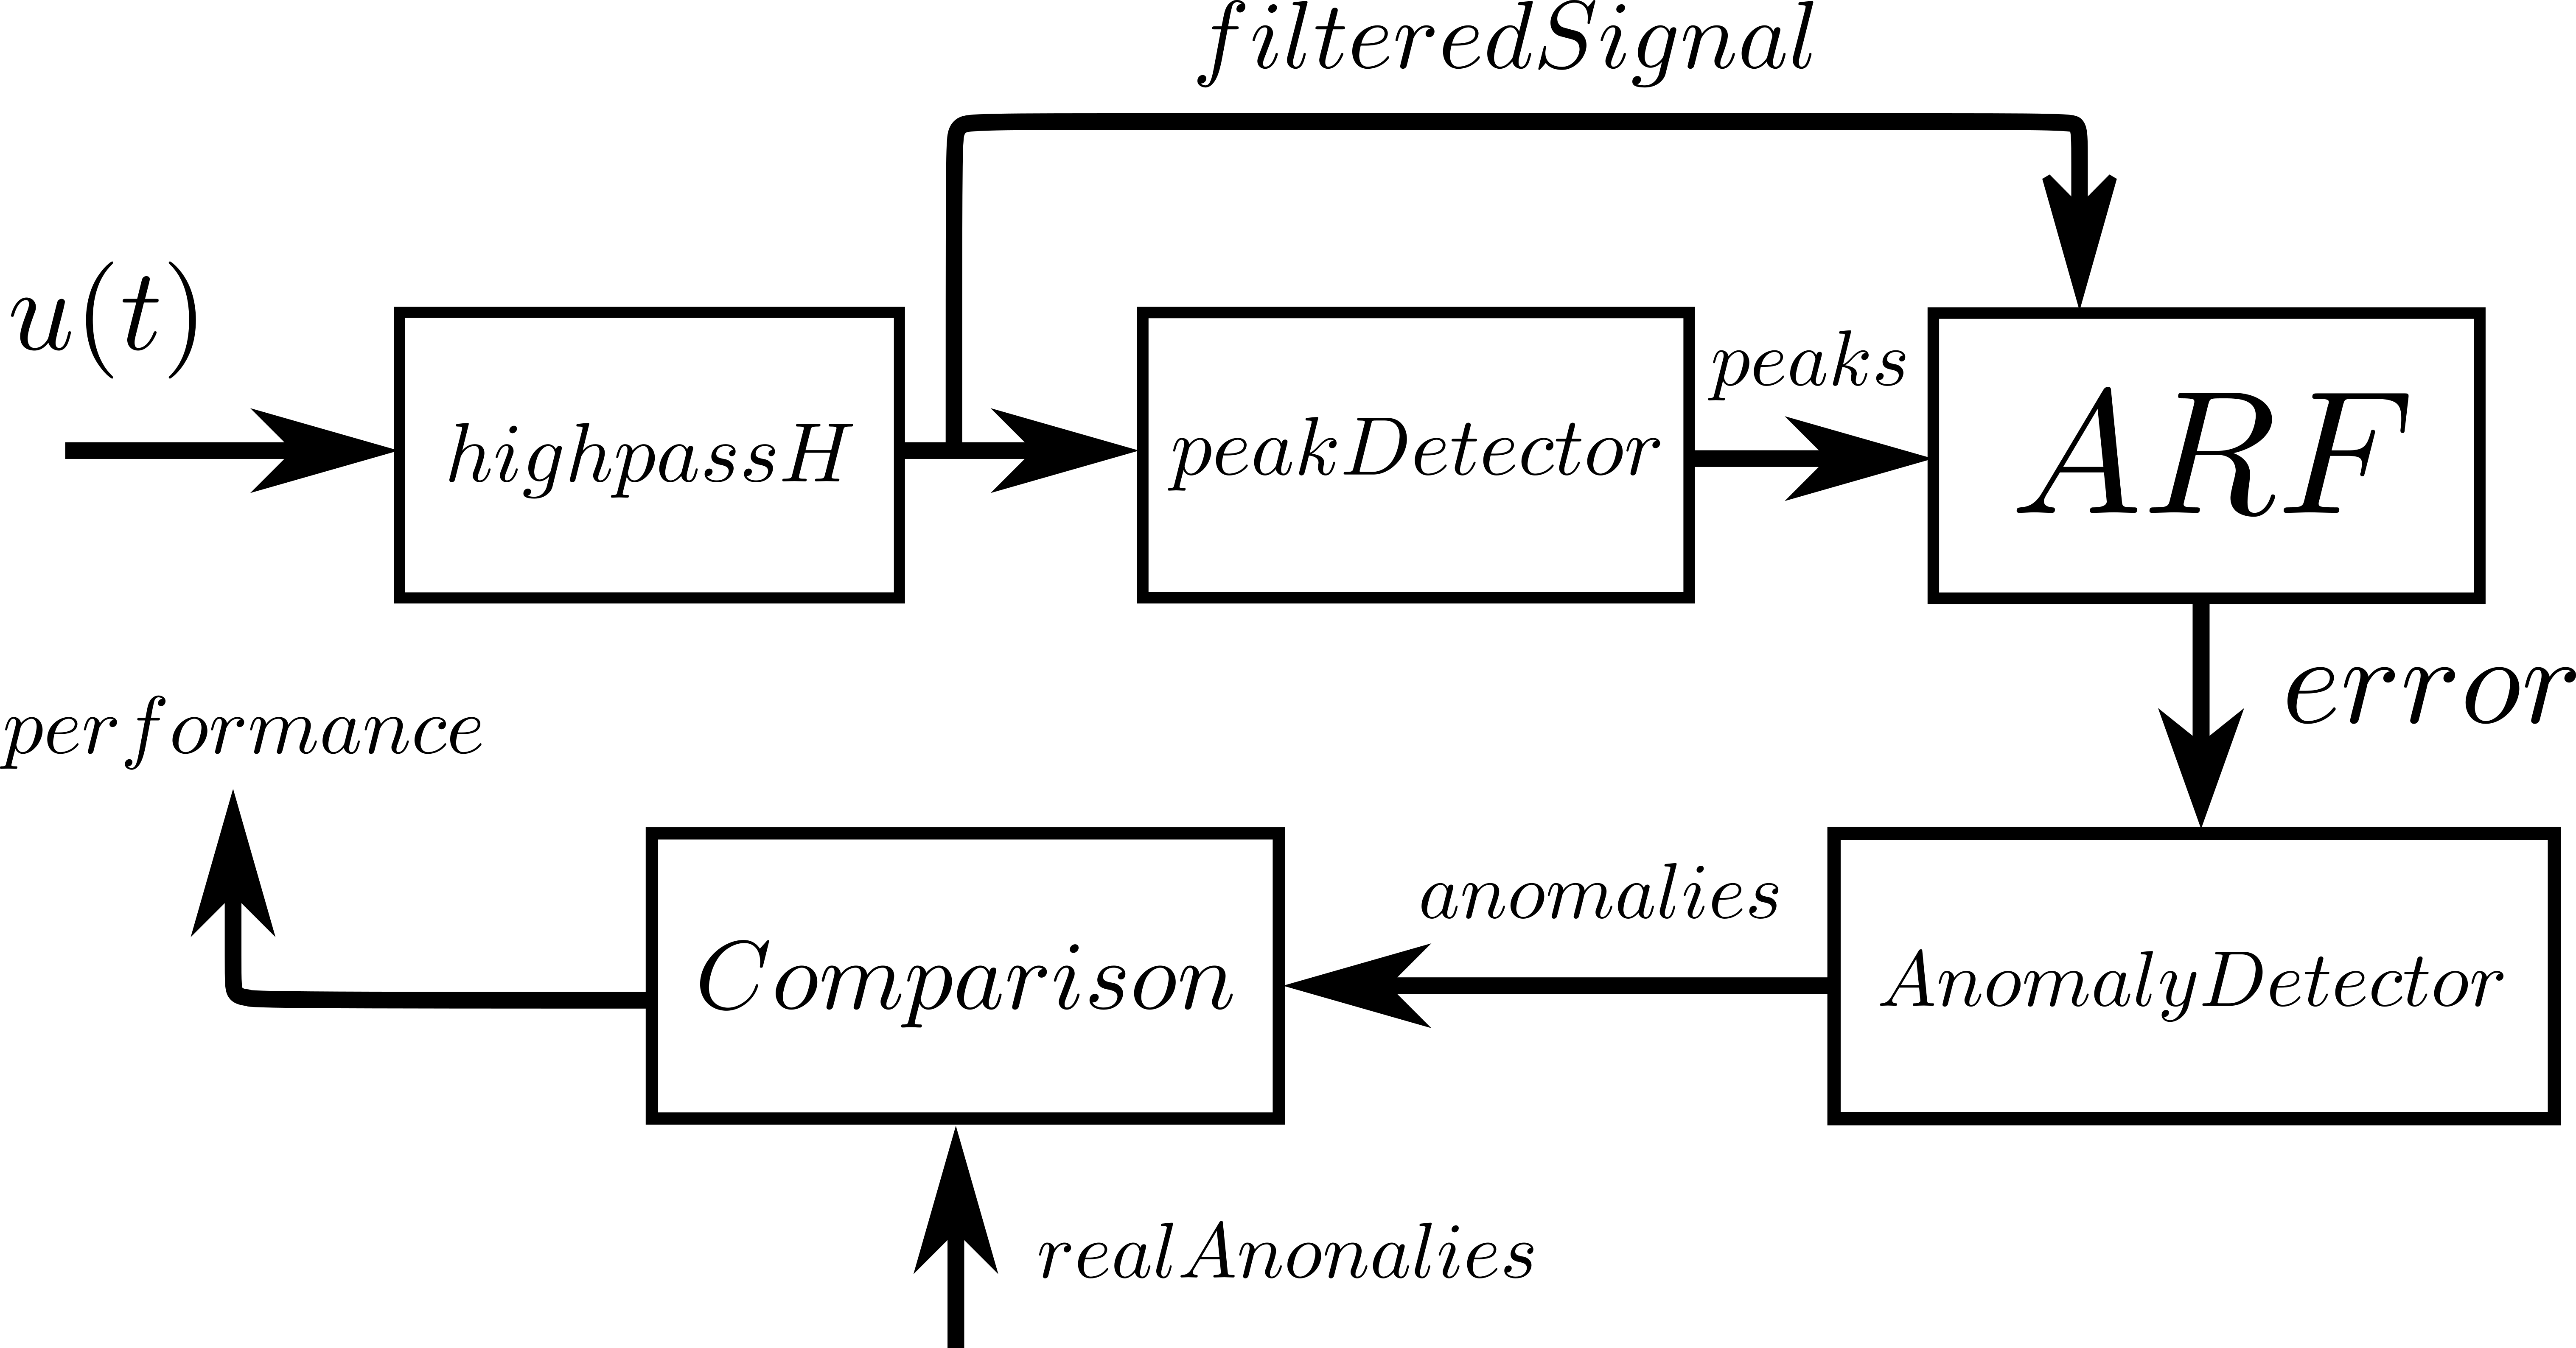
\includegraphics[scale=0.55]{imagenes/diagram}}
\caption{Global system overview}
\label{fig}
\end{figure}
To develop our algorithm we could make another peak detector, but, in practice from the studied signals we have the insight that the energy of the error signal between two peaks is more accurate to detect if there is an anomaly in that region, that is because electrocardiogram failure is more a distributed problem over the whole signal, rather than a localized event.

Our algorithm checks over each region the energy of the signal and if it is sufficiently high (higher than a calibrated value by trial and error) it report a failure. To assign an epicenter (thus being able to compare our algorithm with real anomalies detected by doctors, we used a weighted average.

\begin{figure}[H]
\centerline{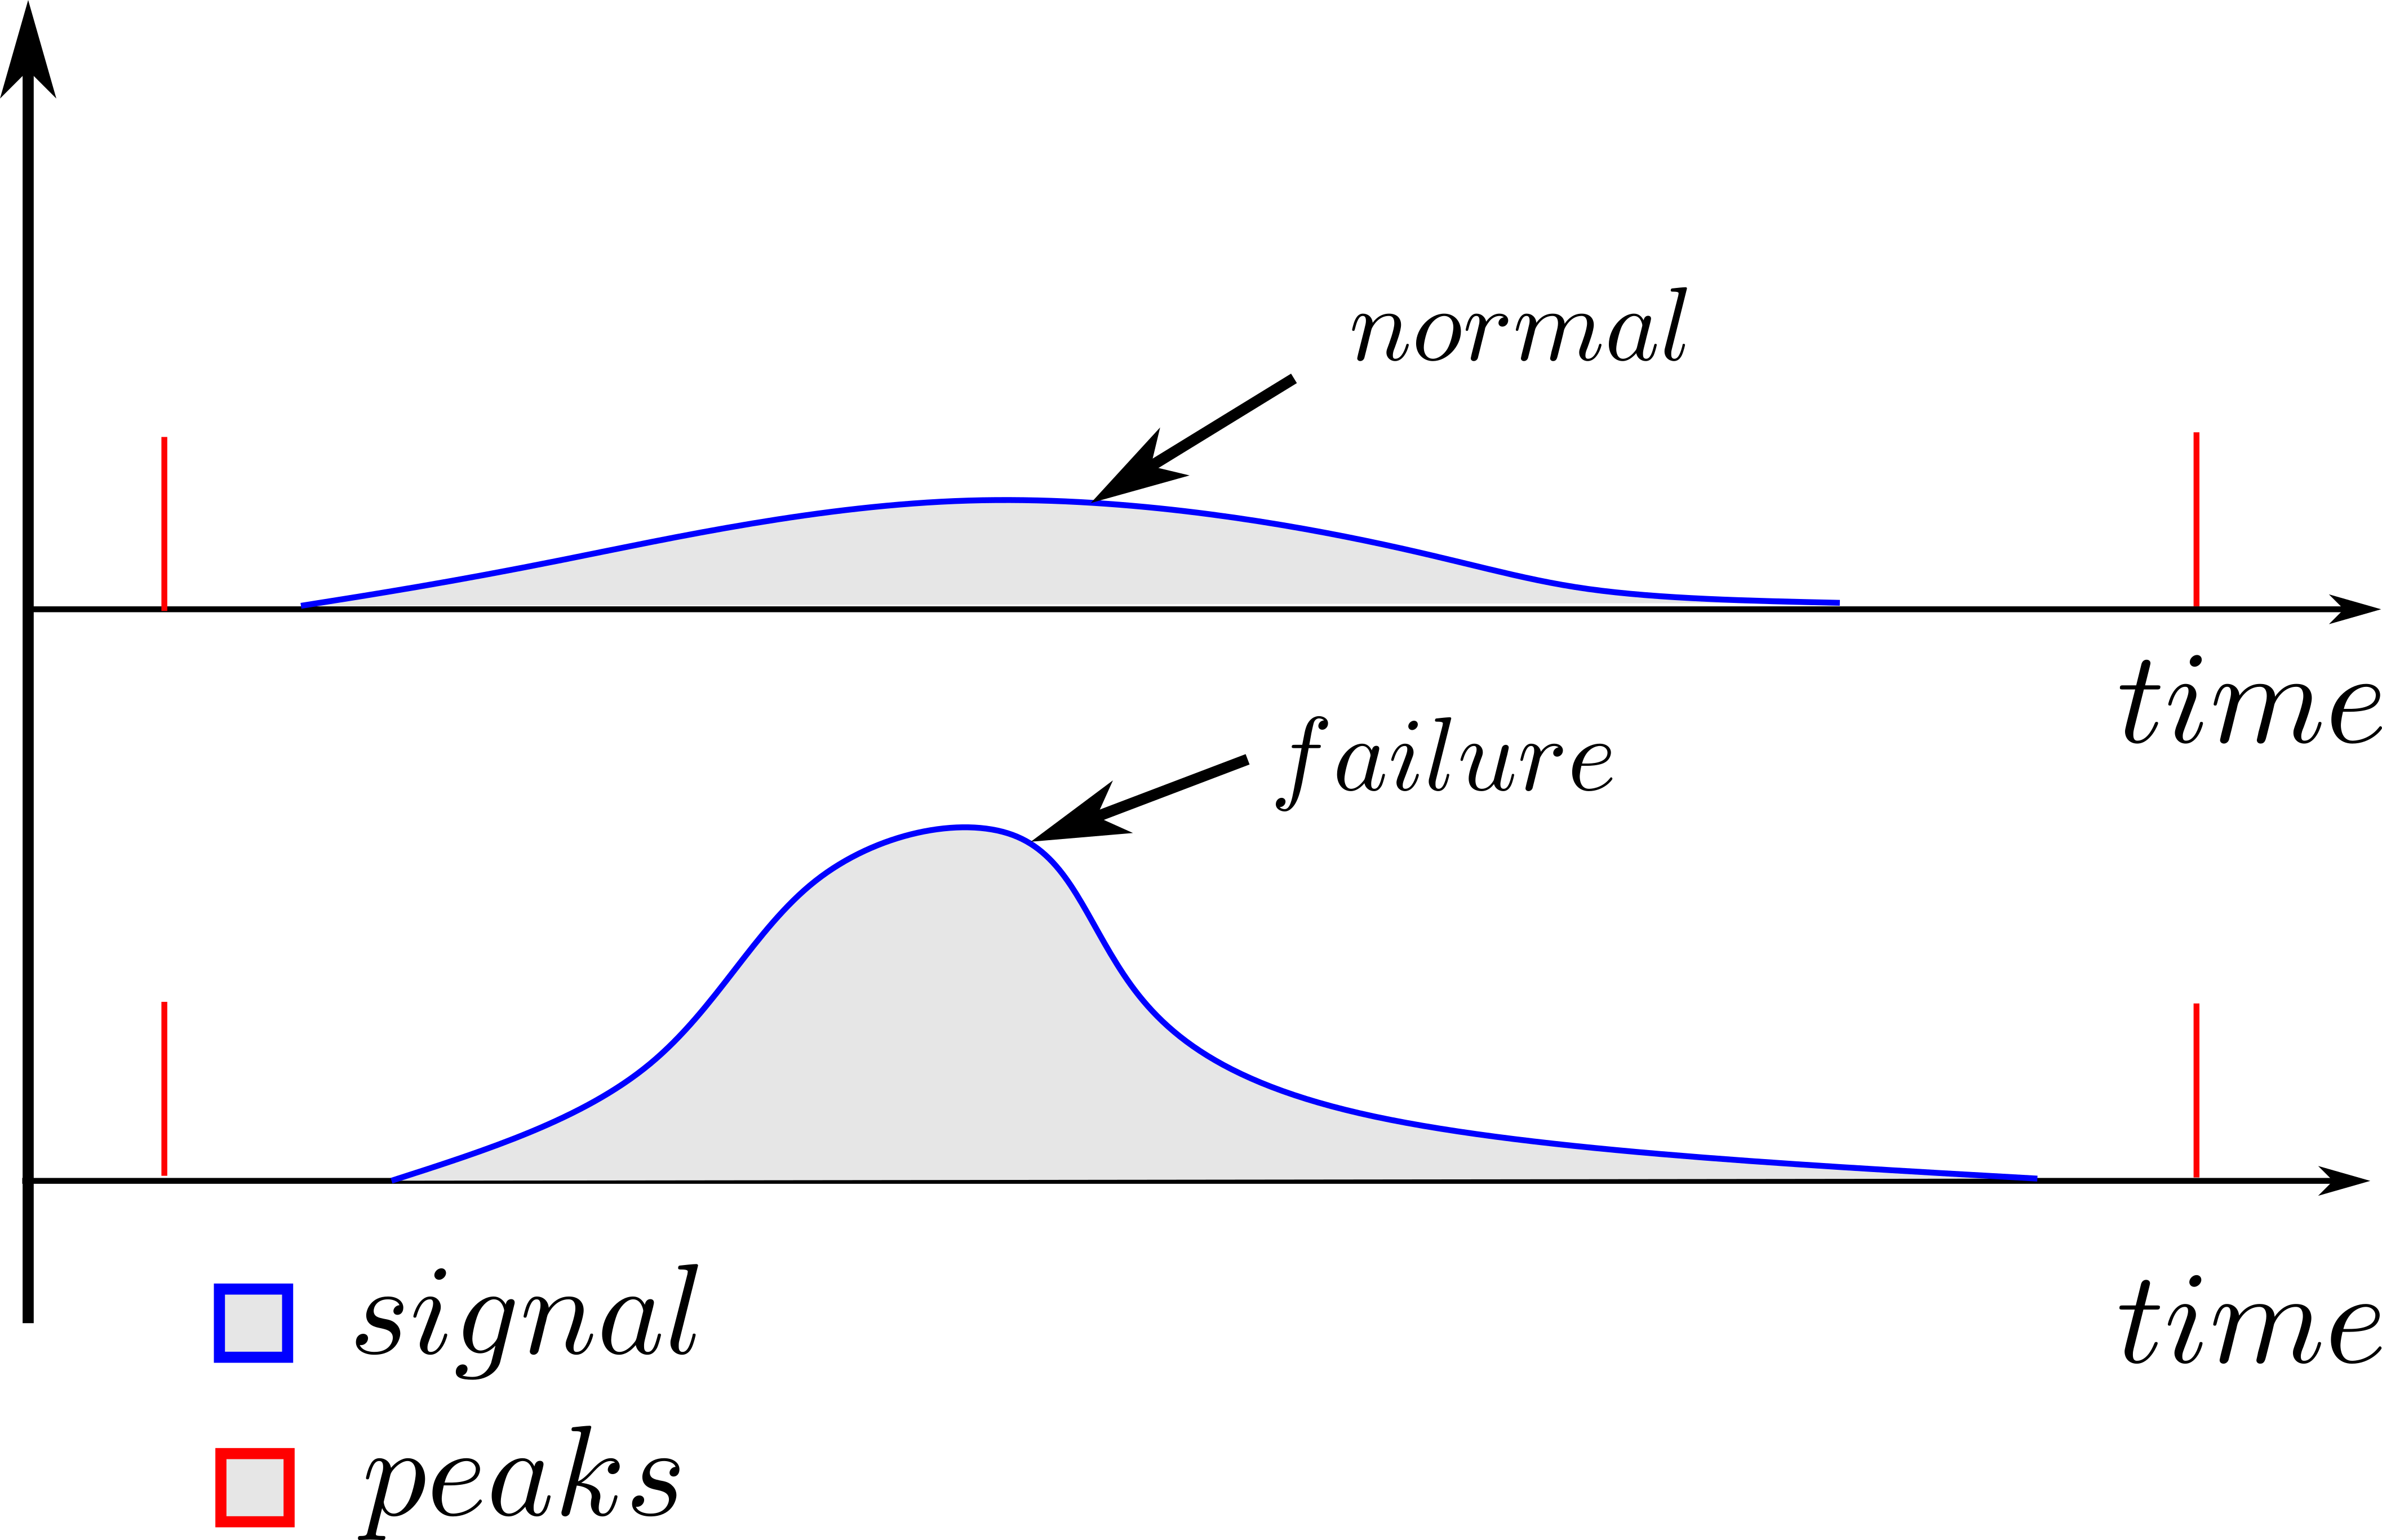
\includegraphics[scale=0.7]{imagenes/anomalyAlgo}}
\caption{Anomaly detection algorithm}
\label{fig}
\end{figure}

We obtained apparently good results in some signals of the database, but pretty bad in anothers. So we developed an Accuracy test to measure how good is our method and in which cases it tend to fail.

\section{Accuracy test}
We had data of the real heart failure times, so we needed to compare that failure times with our failure algorithm declarations. We made two tests to get accuracy information from two different points of view. First we calculated from all detected positive the amount that were calculated correctly, and the we calculated from all the real positives, how much were correctly detected. Note that two points of view are similar but complementary.
The algorithm consisted of an iteration over the detected failure points that checked if a real failure was in range. We computed an array to optimize that calculation.
We have run the accuracy test with all signals.

\begin{figure}[H]
\centerline{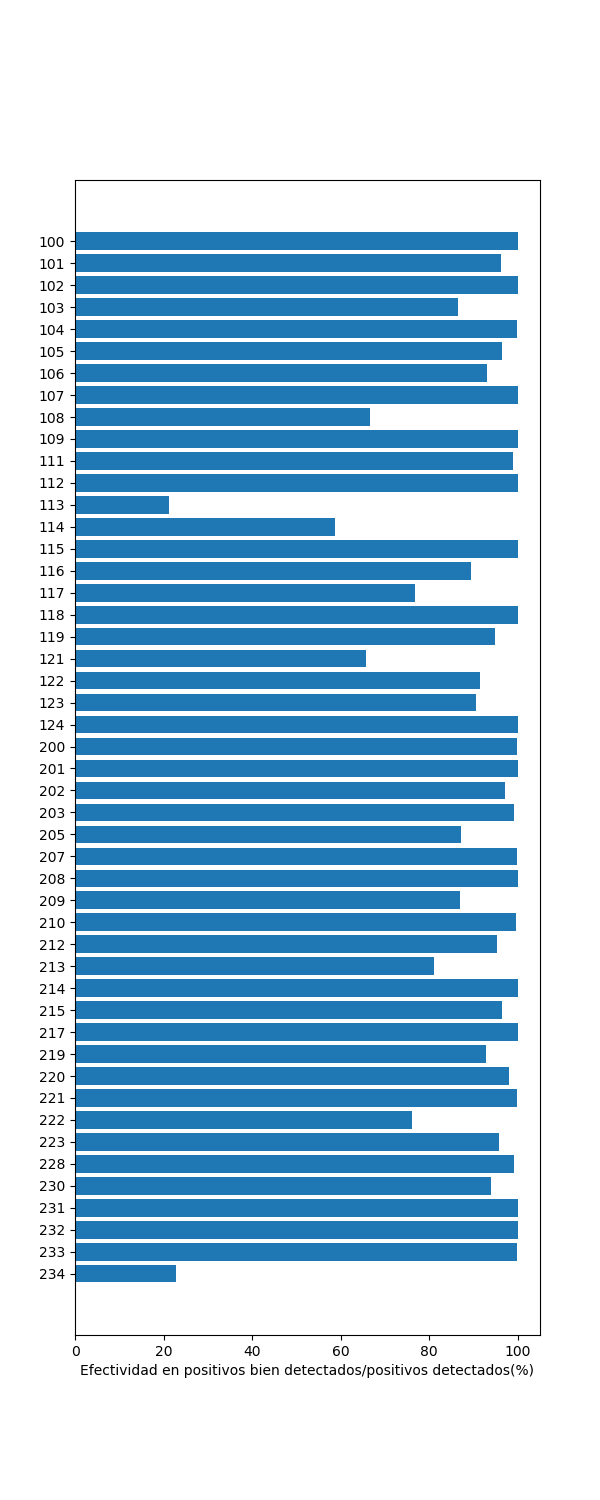
\includegraphics[scale=0.4]{imagenes/EfectividadDetectados}}
\caption{Correctly detected/Detected}
\label{fig}
\end{figure}

\begin{figure}[H]
\centerline{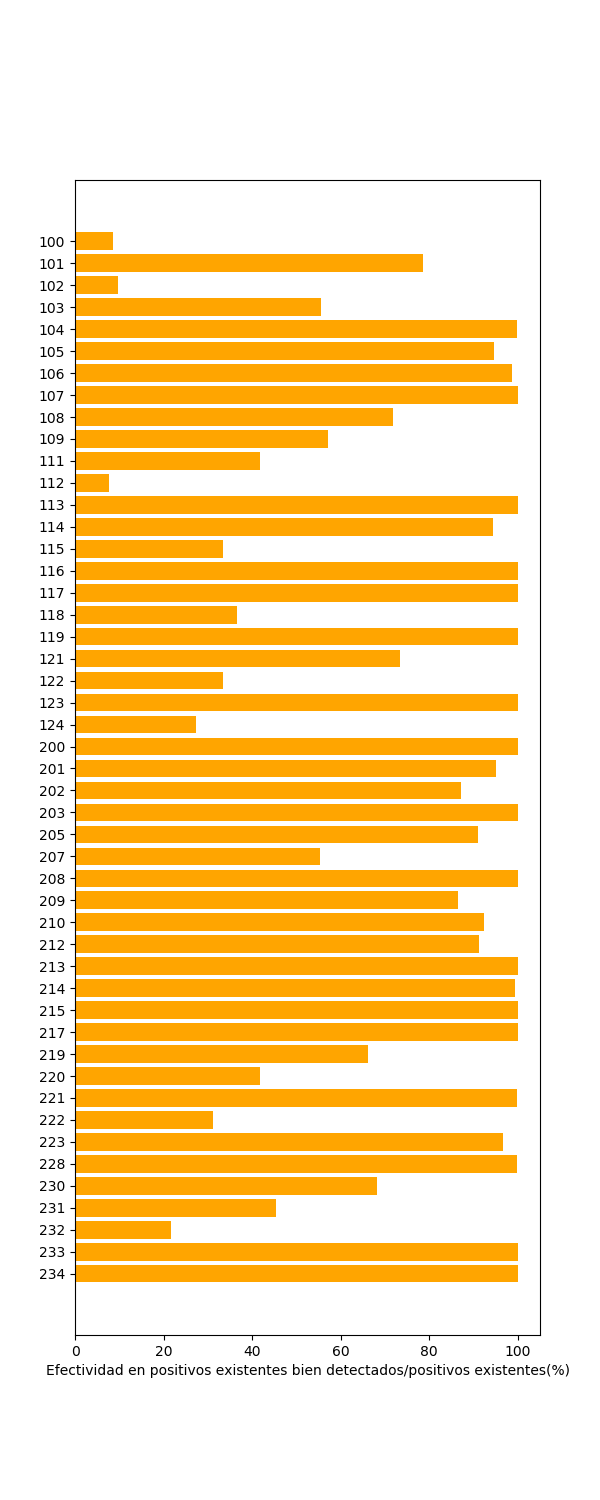
\includegraphics[scale=0.4]{imagenes/EfectividadExistentes}}
\caption{Failures detected/Total heart failures}
\label{fig}
\end{figure}

These two figures are the results.

\section{Analysis and validation of results}


\begin{thebibliography}{00}
\bibitem{b1} Nitish V. Thakor and Yi-Sheng Zhu, ``Applications of Adaptive Filtering to ECG Analysis :
Noise Cancellation and Arrhythmia Detection'', IEEE Transactions On Biomedical Engineering. Vol. 18. No 8. August 1991.
\bibitem{b2} J. A. Van Alste and T. S. Schilder``Removal of Base-Line Wander and Power-Line Interference from the ECG by an Efficient FIR Filter with a Reduced Number of Taps'', IEEE TRANSACTIONS ON BIOMEDICAL ENGINEERING, VOL. BME-32, NO. 12, DECEMBER 1985.
\end{thebibliography}
\end{document}
